\documentclass[10pt,a4paper]{article}

% Import packages
\usepackage[utf8]{inputenc}
\usepackage{amsmath}
\usepackage{amsfonts}
\usepackage{amssymb}
\usepackage{xcolor}
\usepackage[compact]{titlesec}
% Decrease font of subsections
\titleformat{\section}
  {\normalfont\fontsize{12}{15}\bfseries}{\thesection}{1em}{}
\titleformat{\subsection}
  {\normalfont\fontsize{10}{10}\bfseries}{\thesubsection}{1em}{}
  
\usepackage{float}
\usepackage{algorithm2e}
\usepackage{graphicx}
\usepackage[left=2cm,right=2cm,top=2cm,bottom=2cm]{geometry}

% Inhoud van titelpagina
\author{Quinten Bruynseraede  \\ R0674455 \and Louis Van Looy \\ R0861408}
\title{The Ethereum network: a graph analysis}

% Kolomlayout
\usepackage{multicol}
\setlength{\columnsep}{1cm}

% Gebruik \todo{x} voor rode tekst
\newcommand{\todo}[1]{\textcolor{red}{#1}}
\begin{document}

% Voeg title en authors vanboven in
\maketitle

% Abstract 
\begin{abstract}
	Lorem ipsum dolor sit amet, consectetur adipiscing elit. Vestibulum laoreet dapibus purus. Maecenas eleifend, ipsum eget pretium blandit, nibh diam fermentum turpis, quis semper urna orci eget dolor. Aliquam at vehicula odio. Sed facilisis, odio vitae faucibus consequat, nisi metus condimentum leo, et malesuada sapien metus nec odio. Etiam vel orci non dolor interdum ultricies. Nullam in justo dui. Aenean ut eros non felis molestie lacinia eget ut turpis. Mauris malesuada efficitur libero, at volutpat arcu imperdiet ac. Vivamus gravida sodales felis, varius ultrices magna luctus sit amet. Donec blandit ante neque, at blandit dui vestibulum in. Nam vel lorem. 
\end{abstract}

\begin{multicols}{2}

Een paar handige commando's:
\begin{itemize}
\item{\begin{verbatim}\todo{x}\end{verbatim} Maakt rode tekst: \todo{x}}
\item{\begin{verbatim}\section{sectienaam}\end{verbatim}Maak een nieuwe sectie}
\item{\begin{verbatim}\subsection{sectienaam}\end{verbatim}Maak een nieuwe subsectie}
\item{\begin{verbatim}\textbf{tekst}\end{verbatim}Zet tekst in \textbf{bold}}
\item{\begin{verbatim}\textit{tekst}\end{verbatim}Zet tekst in \textit{italics}}
\item{\begin{verbatim}\cite{referentie-naam}\end{verbatim}Maakt verwijzing naar bron (gedefinieerd in references.bib}
\item{\begin{verbatim}\begin{itemize}
\item{item1}
\item{item2}
\end{itemize}\end{verbatim}Maakt een opsomming met bolletjes}
\item{\begin{verbatim}\begin{enumerate}
\item{item1}
\item{item2}
\end{enumerate}\end{verbatim}Maakt een opsomming met nummers}

\end{itemize}

% Nieuwe sectie met \section
\section{Introduction}
The Ethereum network is a blockchain-based network for distributed processing. It contains a thriving ecosystem of distributed applications (dapps), ranging from financial tools to games and gambling. Ethereum's native token is called Ether (ETH), and it has become a acknowledged way of storing and transferring money: a so-called \textit{store-of-value}. In this report, we analyze how ETH is distributed among users, and how it flows between them. In particular, we analyze the role of a group of very wealthy users (called \textit{whales}), and we investigate how important these whales are for the network, and to what degree they contribute to wealth inequality.

In Chapter 2, we introduce some basic concepts related to the ethereum network. Chapter 3 outlines past work about network analysis of cryptocurrency networks, in particular the Ethereum network. In Chapter 4, we describe how we collected the necessary data. Chapter 6 analyzes the network using a set of network analysis tools, and try to show the importance of whales. Chapter 7 focuses on inequality within the Ethereum network. In Chapter 8, we try to analyze clusters in the network, and try to link these clusters to their utility in the network. 

\section{Ethereum}
% Subsections

In the following section, we explain fundamental terms and definitions needed to understand the Ethereum network. Based on this, it is also intended to better understand the network and thus observe and understand the specific characteristics of the particular network. 

\subsection{Ethereum}
First of all a formal definition of Ethereum is needed. Ethereum is an open-source, blockchain-based and decentralized software platform. It makes use of its own cryptocurrency, called Ether. The main novelty of Ethereum is its ability to execute smart contracts and create decentralized, distributed applications without any downtime, fraud, control or involvement from a third party. A smart contract can be seen as a piece of code that describes the rules for a transaction between two parties. Smart contracts on the Ethereum network are Turing-complete (i.e. they can describe arbitrary computations), and are mostly programmed in the Solidity programming language. 
\subsection{Addresses and transactions}
Users store their Ether in an account, uniquely represented by a 20-byte address, such as \texttt{0xed9a430d9a11616eb1cb07ebc28c9e20a03bd486}. Transactions contain (among other fields), a sender, a recipient and a transaction value expressed in \textit{wei}. 1 Ether is equal to 10e\textsuperscript{18} wei. Smart contracts are also identified by a 20-byte address, and executing these smart contracts can be done by sending them a transaction. All transactions are public by default, but there is no direct link between the identify of a user and his address: the vast majority of transactions happen anonymously. However, many services use addresses that are publicly known. For example, Binance, one of the largest cryptocurrency marketplaces, has at least 20 known addresses \footnote{https://etherscan.io/accounts/label/binance}.
\subsection{Whales}
An important element within the composition of the Ethereum network are whales. Ma (2021) gives the following definition: “The term \textit{whale} is used to describe an individual or organization that holds a large amount of a particular cryptocurrency.” This amount is not clearly defined, but within the Ethereum community, addresses that have more than 10 000 Ether are often considered whales. At the time of writing, 10 000 ETH is worth over 22 million USD. The name 'whale' originates from the fact that these addresses have a lot of power on the network and are able to push the market up or down. A whale is not necessarily limited to an individual, it could also refer an institution or organization that holds a significant amount of Ether (Ma, 2021).
\subsection{The network}
The Ethereum network has seen tremendous growth since its inception in 2015, and contains over 350 million transactions at the time of writing. Since June 2020, the daily number of transactions exceeds 1 million \footnote{https://etherscan.io/chart/tx}. Over 100 million addresses have been registered, and over 600 thousand addresses take part in transactions every day \footnote{https://bitinfocharts.com/comparison/ethereum-activeaddresses.html}. This means a full analysis is generally not feasible.

\section{Related Work}
\todo{TODO}
\section{Data collection}
Given the size of the Ethereum network, we have to resort to sampling techniques. One type of sampling uses \textit{random walks}, that start at a given point and follow edges while collecting the necessary data. Random walks are particularly useful for networks where it is not possible to delimit a part of the network in advance \cite{Becchetti06acomparison}. Ethereum is such a network: addresses are not ordered or structured in any way. We collect transactions using a Breadth-first search (BFS). To analyze the evolution of the network, we create separate 6 snapshots: each snapshot contains 1 million transactions that span 1 month of time.

\medskip
\begin{algorithm}[H]
\SetAlgoLined
\hspace{5pt}\texttt{T} = $\emptyset$\newline
Initialize \texttt{Queue} with 100 known addresses
\While{\texttt{T.size} $\leq$ 1e6}{
\hspace{5pt}1. Pop an address \texttt{A} from \texttt{Queue}\newline
2. Fetch all transactions by \texttt{A} during the time period \newline
3. Add all transactions to \texttt{T} \newline
4. Add all addresses that occur in these transactions to \texttt{Queue }\newline 
} 
\end{algorithm}

Although transactions contain many more features, we only use the columns \texttt{from}, \texttt{to}, and \texttt{value}.

\section{Analysis of the Ethereum network}
\todo{TODO}
	
\begin{figure}[H]
\centering
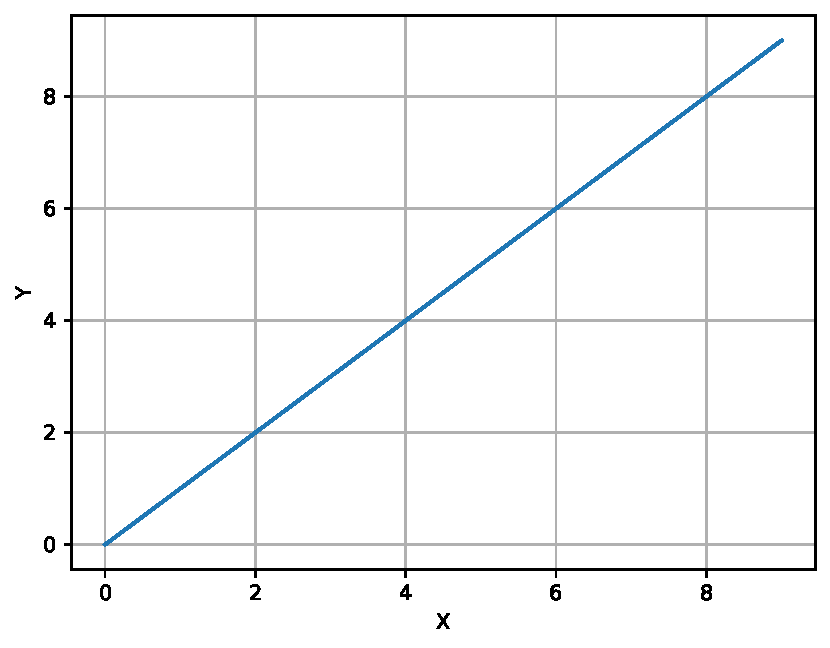
\includegraphics[scale=0.44]{figures/graph.pdf}
\caption{A graph}
\label{fig-agraph}
\end{figure}

Hier verwijs ik automatisch naar Figure \ref{fig-agraph}. \\
\section{Inequality}
\todo{TODO}
\section{Clustering}
\end{multicols}
\bibliographystyle{plain}
\bibliography{references}
\end{document}
